%%%%%%%%%% Merge with supplemental materials %%%%%%%%%%
%%%%%%%%%% Prefix a "S" to all equations, figures, tables and reset the counter %%%%%%%%%%
\setcounter{equation}{0} %Resets page, eqn, figure, table numbers
%\setcounter{figure}{0}
%\setcounter{table}{0}
%\setcounter{page}{1} 
\makeatletter
\renewcommand{\theequation}{S\arabic{equation}} %Adds S to the front of references
\renewcommand{\thefigure}{S\arabic{figure}}
\renewcommand{\thetable}{S\arabic{table}}
\renewcommand{\bibnumfmt}[1]{[S#1]}
\renewcommand{\citenumfont}[1]{S#1}
%\pagenumbering{gobble}

\pagebreak
%\widetext
\begin{center}
\textbf{\large Appendix A: Additional figures and tables}
\end{center}

% \begin{figure}
%     \centering
%     \includegraphics[width=\textwidth,keepaspectratio=true]{fieldMap.eps}
%     \caption{Map of sampled fields, showing locations of 29 commodity canola fields (14 during 2014, 15 during 2015), and 35 seed canola fields (15 during 2015, 20 during 2016). Seed canola is grown only in southern Alberta, while commodity canola is grown across both the northern and southern regions.}
%     \label{fig:fieldMap}
% \end{figure}


\begin{figure}
    \centering
    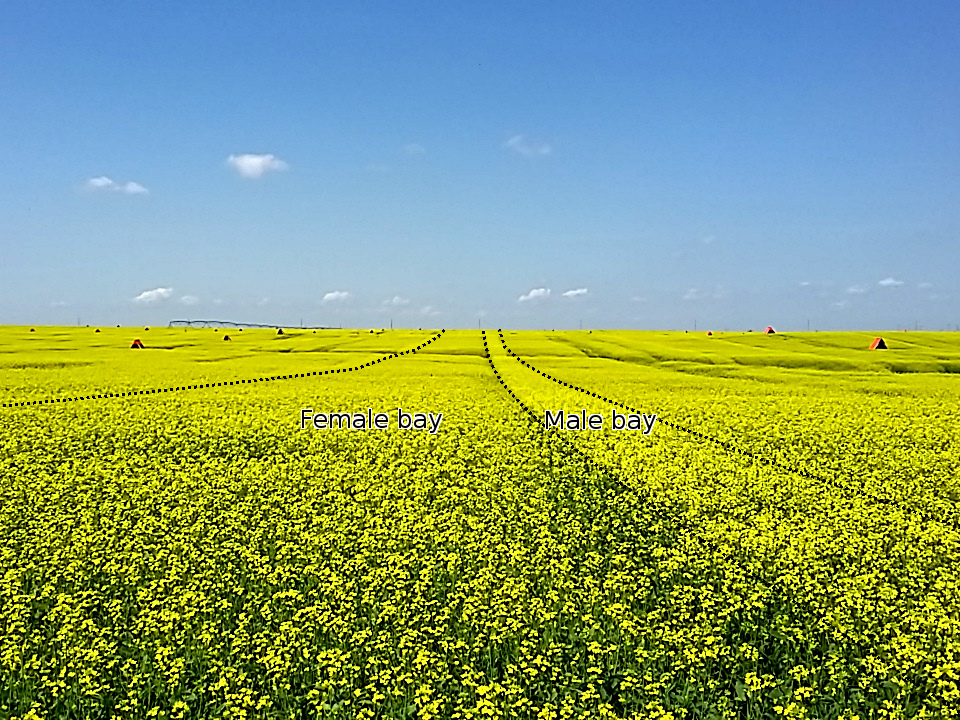
\includegraphics[width=\textwidth,keepaspectratio=true]{seedfieldBays.jpg}
    \caption[Hybrid seed field near Rainer, AB]{Hybrid seed field near Rainer, AB, showing the outlines of male and female bays in the foreground, with orange leafcutter bee shelters stationed throughout the field. The linear structure on the horizon is the central-pivot irrigation sprinkler.}
    \label{fig:seedfieldPhoto}
\end{figure}

\begin{figure}
    \centering
    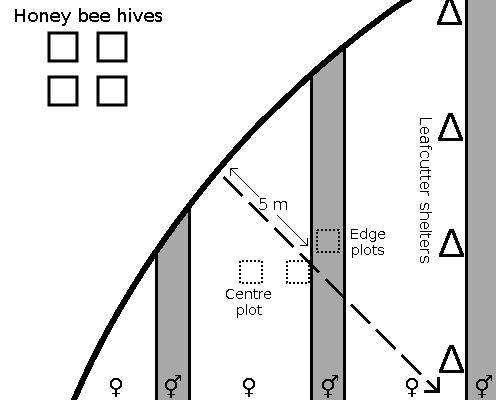
\includegraphics[width=0.6\textwidth,keepaspectratio=true]{seedfieldPlots.png}
    \caption[Plot arrangement for surveys in hybrid seed fields]{Plot arrangement for surveys in hybrid seed fields, showing hypothetical arrangement of leafcutter shelters ($\Delta$), and male-fertile (\Hermaphrodite) and female bays (\Female) at 5m from the edge of the field. Plots were placed 5, 20, 100, and 400m along a transect (dashed line) from the field edge nearest to the set of honey bee hives. Plots were placed side-by-side in the male bay and edge of the female bay (``edge" plots), and at the 5m and 400m distances, a plot was placed in the centre of the female bay (``centre" plots).}
    \label{fig:seedfieldPlots}
\end{figure}


\begin{figure}
	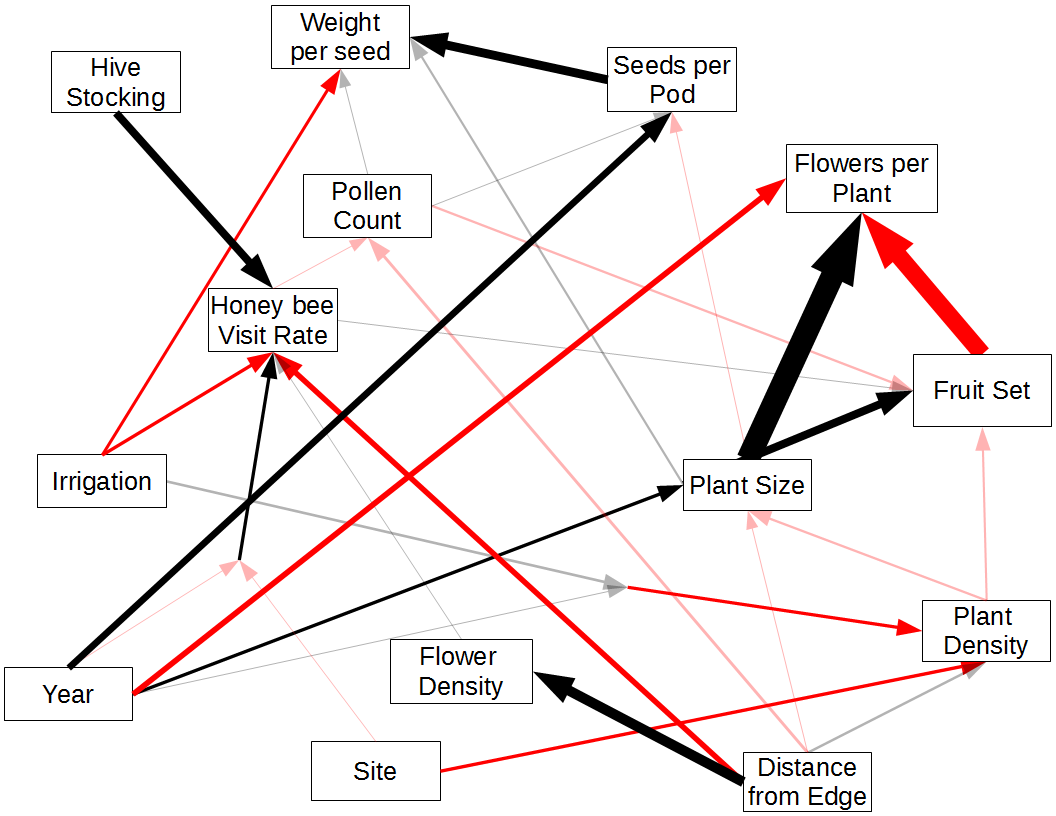
\includegraphics[width=\textwidth,keepaspectratio=true]{commodity_sem.png}
    \caption[Path diagram for commodity canola model]{Path diagram for the commodity canola model, with positive and negative terms shown in black and red, respectively. Line thicknesses are proportional to effect size (mean/SD) of coefficients. Coefficients with 95\% posterior quantiles overlapping zero are shown with a transparent line. Interactions are shown as an inverse Y-shaped path, with the two branches representing main effects, and the final branch representing the interaction term (\textit{e.g.} effect of site and year on honey bee visitation rate). Year:site interaction is also shown in Figure \ref{fig:hbeeDist_commodity}. ``Year" indicates the year effect of 2015, and ``Site" indicates the site effect of Grande Prairie.}
    \label{fig:commoditySEM}
\end{figure}

\begin{figure}
	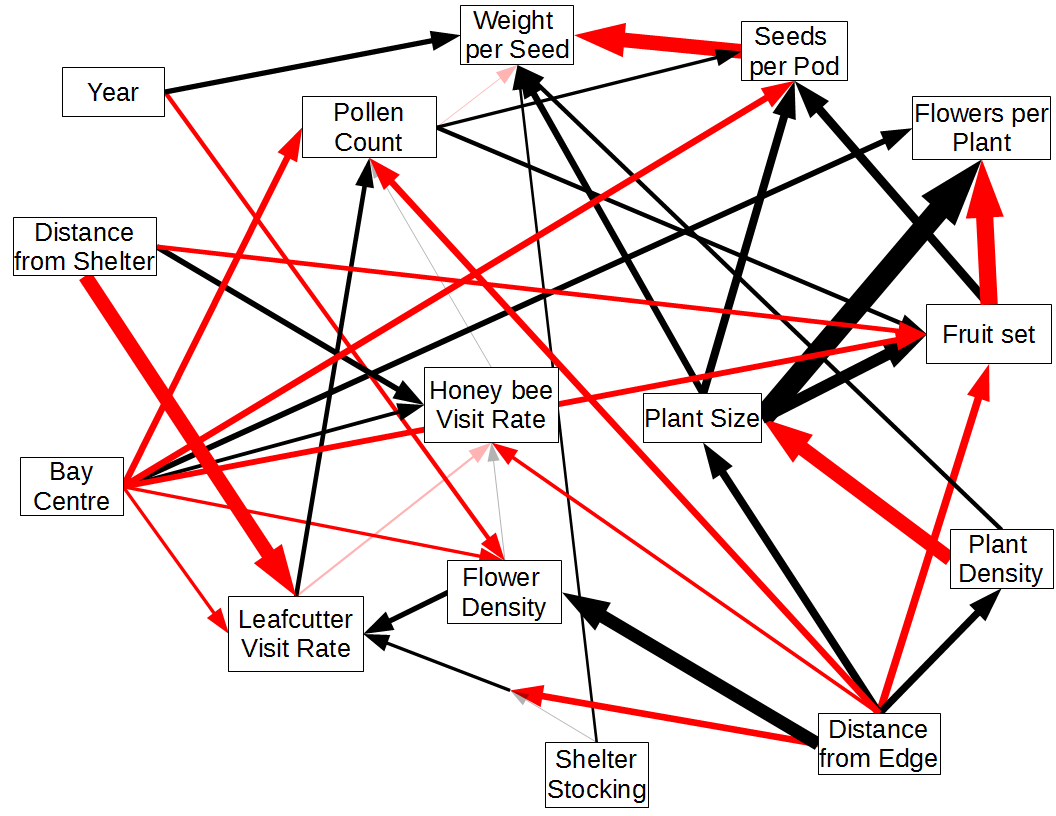
\includegraphics[width=\textwidth,keepaspectratio=true]{seed_sem.png}
    \caption[Path diagram for seed canola model]{Path diagram for the seed canola model with positive and negative terms shown in black and red, respectively. Line thicknesses are proportional to effect size (mean/SD) of coefficients. Coefficients with 95\% posterior quantiles overlapping zero are shown with a transparent line. Interactions are shown as an inverse Y-shaped path, with the two branches representing main effects, and the final branch representing the interaction term (\textit{e.g.} effect of distance from edge and shelter stocking rate on leafcutter bee visitation rate). Stocking:Distance interaction is also shown in Figure \ref{fig:hbeeDist_both}. ``Year" indicates the year effect of 2015.}
    \label{fig:seedSEM}
\end{figure}